\section{Marco Teórico}

\subsection{Validación de Modelos}
Los modelos son representaciones matemáticas de los mecanismos que rigen los fenómenos naturales \parencite{tedeschi-2006} o como una construcción matemática diseñada para estudiar un sistema del mundo real o fenómeno (Giordano et al., 1997).\\

\textcite{medina-peralta-2017} indican que la validación de un modelo en la predicción del sistema implica la comparación, por medio de algún método, de las predicciones del modelo con los valores observados del sistema real para determinar su capacidad predictiva.\\

\textcite{mayer-butler-1993}, clasifican los métodos de validación de modelos en Evaluación Subjetiva, Técnicas Visuales, Medidas de Desviación y Pruebas Estadísticas; también señalan que debido a las complejidades y tipos de datos, no existe una combinación establecida de técnicas de validación que sea aplicable en todas las áreas.\\

Halachmi et al. (2004), menciona que la validación determina si el modelo matemático es una representación exacta del sistema real, y una forma de validación es comparando los datos reales con los predichos por el sistema.
\vspace{.5cm}

Para la validación de un modelo se evalúan la exactitud y la precisión; la primera se refiere a la proximidad de las predicciones $( z )$  con los valores observados $( y )$, por ejemplo, sus diferencias $ ( d=y-z ) $ del cero y la segunda a la dispersión de los puntos $ (z, y) $; además, en presencia de exactitud la precisión se mide cuantificando la dispersión de dichos puntos respecto a una referencia, por ejemplo, la recta determinística  $ y=x $, o bien, evaluar la varianza de las diferencias $ (\sigma_{D}^{2}) $ alrededor del cero $ (\mu_{D}=0) $ \parencite{medina-peralta-2017}.
\vspace{.5cm}

En la Figura \ref{fig:EsquemaExacPreci} se ilustra la diferencia entre la exactitud y precisión de un modelo de simulación. El caso 1 es inexacto e impreciso, el caso 2 es inexacto y preciso, el caso 3 es exacto e impreciso y el caso 4 es exacto y preciso. En un modelo de predicción lo ideal es que cumpla el caso 4. 

\begin{figure}[H]
	\centering
	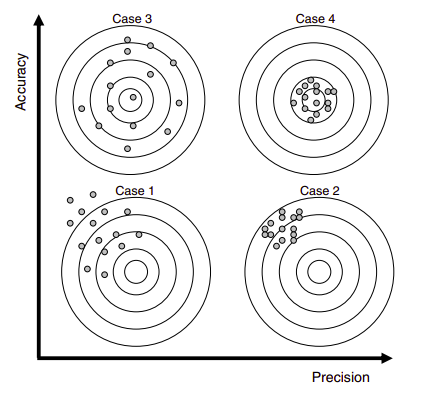
\includegraphics[width=180px]{img/tadeshi_casos.png}
	\caption{Esquematización de Exactitud y Precisión. Fuente: Tedeschi (2006).}
	\label{fig:EsquemaExacPreci}
\end{figure}
\FloatBarrier

De manera similar, la Figura \ref{fig:ComparmedidExacPreci} representa los conceptos ilustrados en la Figura \ref{fig:EsquemaExacPreci} en una forma numérica; el eje $X$ y el eje $Y$ representan al modelo de los valores predichos contra los observados respectivamente. El caso 1 es inexacto e impreciso, el caso 2 es inexacto y preciso, el caso 3 es exacto e impreciso y el caso 4 es exacto y preciso. La línea punteada representa la línea de $X = Y$ . En un modelo de predicción lo ideal es que cumpla el caso 4. 

\begin{figure}[H]
	\centering
	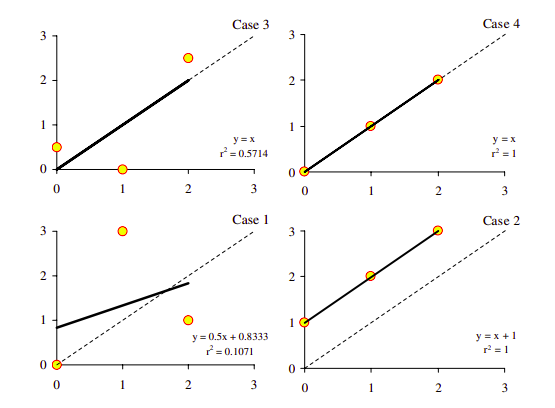
\includegraphics[width=0.6\linewidth]{img/tedeshi_casos_2.png}
	\caption{ Comparación de las medidas de Exactitud y Precisión. Fuente: Tedeschi (2006).}
	\label{fig:ComparmedidExacPreci}
\end{figure}
\FloatBarrier

Las estimaciones del intercepto y la pendiente son buenos indicadores de la exactitud: cuanto mas cerca
estén simultáneamente de cero y uno respectivamente mayor es la exactitud. La estimación del coeficiente de
determinación $(R^{2})$ es un buen indicador de la precisión: cuanto mayor es la $R^{2}$ mayor es la precisión \parencite{balam-2012}.
\vspace{.5cm}

Por su parte, \textcite{mayer-butler-1993} indican que la prueba $t$ paramétrica de medias y el análisis de regresión lineal de la grafica observada frente a la predicha son los métodos estadísticos generales mas útiles, sin embargo, cada método inferencial se encuentra principalmente sujeto a las dificultades para satisfacer sus supuestos.
\vspace{.5cm}



\subsection{Validación de Modelos con Regresión Lineal}
Una de las técnicas mas comunes en la validación de modelos es la de Regresión Lineal Simple de los observados sobre los predichos (Mayer et al., 1994; Analla, 1998; Tedeschi, 2006).
\vspace{.5cm}


El análisis de regresión lineal tiene como objetivo modelar en forma matemática el comportamiento de una variable de respuesta en función de una o mas variables independientes
(Gutiérrez y de la Vara, 2012). Por lo tanto, se ajusta el modelo  $ y_{i} = \beta_{0} + \beta_{1}z_{i} +\epsilon $ donde $ 1 \leq i \leq n$, $ y_{i}$ es el valor real observado en la i-esima unidad experimental, $ z_{i}$ es el correspondiente valor predicho por el modelo a validar, $\epsilon_{i}$ es el componente aleatorio o error, $\beta_{0}$ es la ordenada al origen y $\beta_{1}$ la pendiente \parencite{zacarias-2023}.
\vspace{.5cm}


\textcite{zacarias-2023}, menciona que una parte importante del método de regresión lineal, es que estudia si dicha relación permite realizar estimaciones con una precisión aceptable; por lo que también se considera como un criterio cuantitativo relevante para evaluar la calidad de ajuste de la regresión, el coeficiente de determinación $R^{2}$, que en general se interpreta como la proporción de la variabilidad en los datos observados $y_{i}$, que es explicada por el modelo.
\vspace{.5cm}

En este contexto \textcite{febles-2014} presenta la validación de modelos con la técnica de regresión lineal simple basándose en el trabajo previo de \textcite{balam-2012}, quien describe el proceso de validación de modelos utilizando la técnica.


\subsubsection{Validación de modelos con la técnica de regresión lineal simple \parencite{febles-2014}}

Sea el modelo $Y = H( )$, donde representa un vector de parametros desconocidos.
Suponga que se desea validar este modelo con la tecnica de regresion lineal simple; para
ello se requiere de una muestra pareada (z1 y1) (z2 y2)
(zn yn) de valores observados
y predichos respectivamente por el modelo Y = H( ). Bajo estas condiciones, se considera
el modelo de regresion lineal: $y_{i}= \beta_{0} + \beta_{1}z_{i}$ y esta dado por:


\begin{center}
	$R^{2} = \frac{ \sum_{i=1}^{n} ( \hat{y}_{i} - \bar{y})^{2}} { \sum_{i=1}^{n} ( y_{i} - \bar{y})^{2}  }$  y  $ 0 \leq R^{2} \leq 1$.
\end{center}

















\subsubsection{Coeficiente de Determinación (Balam, 2012) }

Se utiliza cuando las variables de estudio son cuantitativas medidas en escala de intervalo o de razón para medir el ajuste del modelo a los datos. El valor de $R^{2}$ frecuentemente es considerado como la proporción de la variación explicada por el modelo de regresión $y_{i}= \beta_{0} + \beta_{1}z_{i}$ y esta dado por:


	\begin{center}
	$R^{2} = \frac{ \sum_{i=1}^{n} ( \hat{y}_{i} - \bar{y})^{2}} { \sum_{i=1}^{n} ( y_{i} - \bar{y})^{2}  }$  y  $ 0 \leq R^{2} \leq 1$.
\end{center}


















\subsection{Regresión Lineal Robusta}
Los estimadores de regresión robusta son una alternativa a los estimadores de mínimos cuadrados cuando no se cumplen los supuestos de normalidad y el de varianza constante en un modelo de regresión lineal, ya que están diseñados para no ser afectados por valores atópicos o por alguna discrepancia en las hipótesis del modelo. La regresión robusta tiene como objetivo derivar métodos que produzcan inferencias confiables para los parámetros del modelo. Existe una gran variedad de estimadores robustos para los coeficientes de regresión, por lo que al elegir uno de ellos se toma en cuenta que tenga ciertas propiedades deseables como son e ciencia alta, varianza mínima, punto de ruptura alto y un mayor
ajuste exacto mínimo. El punto de ruptura es una medida de la robustez del estimador y se define para muestras finitas como la mínima fracción de datos anómalos que puede causar que el estimador no sea útil. El ajuste exacto mínimo se refiere ere al porcentaje mínimo de observaciones que se ajustan exactamente al modelo de regresión. \\


En un principio, el uso de los estimadores robustos era limitado ya que su computo requería de métodos iterativos que son mas complicados que el computo de los estimadores de mínimos cuadrados, pero con el tiempo el uso fue cada vez mayor debido a nuevos algoritmos rápidos de computo y al desarrollo de resultados teóricos que permitieron mejorar la eficacia e incrementar el punto de ruptura, a tal grado de pasar del 0\% al 50\%. Los primeros estimadores robustos propuestos fueron el L1-Estimador y el M-Estimador (Huber, 1973), aunque estos en teoría eran mas apropiados que los estimadores de mínimos
cuadrados cuando no se cumplan los supuestos del modelo de regresión, tenían el mismo punto de ruptura que los mínimos cuadrados, es decir, $1/n$, el cual convergía a cero cuando $ n \rightarrow \infty$. El GM-Estimador se propuso para incrementar el punto de ruptura alcanzando un máximo del 30\% para modelos de regresión simple, aunque para modelos de regresión múltiple su punto de ruptura converge a cero. Adicionalmente, se propusieron estimadores robustos con punto de ruptura máximo del 50\%; como el propuesto por Siegel (1982)
basado en la minimización de la mediana repetida (RM); y los propuestos por Rousseeuw (1984), uno basado en la mínima mediana de los cuadrados de los residuos (LMS) y el otro basado en los mínimos cuadrados recortados de los residuos (LTS). Rousseeuw y Yohai (1984) propusieron los S-Estimadores basados en la minimización de un M-Estimador de la escala residual; sin embargo, todos estos estimadores robustos no son muy eficientes. Actualmente, se cuenta con estimadores robustos de regresión que se construyen por etapas, cuyo computo es mas demandante, sin embargo, logran alcanzar un punto de ruptura
máximo del 50\% y una e ciencia asintótica mayor al 85\%, uno de los mas utilizados es el MM-Estimador.\\

\subsubsection{MM-Estimador (Yohai, 1987)}
El estimador MM tiene las siguientes propiedades: (i) es altamente eficiente cuando los errores tienen una distribución normal y (ii) su punto de ruptura es 0.5.\\

El estimador MM se define en un procedimiento de tres etapas. En la primera etapa, se calcula una estimación de regresión inicial que es consistente, robusta y con un alto punto de ruptura, pero no necesariamente eficiente. En la segunda etapa, se calcula un estimador M de la escala de errores utilizando residuos basados en la estimación inicial. Finalmente, en la tercera etapa se calcula un estimador M de los parámetros de regresión basada en una función $\psi$ descendente.\\

Considerando el modelo de regresión lineal simple:
\begin{center}
$y_{i}= \beta_{0} + \beta_{1}z_{i}$, $1 \leq i \leq n, $
\end{center}

Huber (1981) de ne los estimadores M de la siguiente manera: Sea una función real que satisfaga los siguientes supuestos (A1):

\begin{enumerate}[label=\roman*.]
	\item $\rho(0) = 0$.
	\item   $\rho(-u) =  \rho(u)$.
	\item $1 \leq i \leq v$ implica $\rho(u) \leq  \rho(v)$.
	\item $\rho$ es continua.
	\item Sea a = sup $\rho(u)$, entonces $0<a< \infty$.
	\item Si $\rho(u) < a $ y $0 \leq  u < v $, entonces  $\rho(u) <  \rho(v)$.
\end{enumerate}

Dada una muestra de tamaño $n$, $ \mathbf{u} = (u_{1}, u_{2}, \dots , u_{n})$,  el estimador M, $s(\mathbf{u})$ está de nido como el valor de s que es la solución de\\

\begin{center}
	$\frac{1}{n} \sum_{i=1}^{n} \rho( \frac{u_{i}}{s}) = b$,\\
\end{center}

donde$ b$ puede de definirse como $E_{\Phi}(\rho(u)) = b$, donde $\Phi$ denota la distribución normal estándar.\\

Se cumple que si $c(\mathbf{u}) = \#\{i : 1 \leq i \leq n, u_{i}=0\} / n < 1- (b/a) $, entonces la sumatoria previa tiene solución única y esta solución es diferente de 0. Si $c(\mathbf{u}) \geq 1 -  (b/a)$, se define $s(\mathbf{u}) = 0$. \\

Luego, el estimador MM se define en tres etapas de la siguiente manera:\\

\begin{enumerate}
	\item Sean $ \beta_{0}^{'}$ y $ \beta_{1}^{'}$ estimaciones de los parámetros$ \beta_{0}$ y $ \beta_{1}$ respectivamente con un alto punto de ruptura, posiblemente 0.5.
	\item  Calcular los residuales\\
	\begin{center}
		 $ \epsilon_{i} = y_{i} -\beta_{0}^{'} -\beta_{1}^{'} z_{i}  $, $1 \leq i \leq n $.\\
	\end{center}
	
	y calcular $s_{n} = s(\epsilon_{i})$, el estimador M de nido previamente, usando una función $\rho_{0}$ que satisface los supuestos (A1) y considerando una constante $b$ tal que $b/a = 0.5$, donde$ a = $ máx $ \rho_{0}(u)$, lo cual implica que para esta escala la estimación tiene un
	punto de ruptura igual a 0.5.
	
	\item  Sea $\rho_{1}$ otra función que satisfaga los supuestos (A1) y tal que\\
	$\rho_{1}(u) \leq \rho_{0}(u)$\\
	sup $\rho_{1}(u)$  = sup $ \rho_{0}(u) = a$\\
	
	Sea $\psi_{1} = \rho_{1}^{'}$. Entonces el estimador MM, se define como cualquier solución de\\
	
	$\sum_{i=1}^{n} \psi_{1} (\frac{\epsilon_{i}}{s_{n}}) z_{i} = 0$\\
\end{enumerate}


\subsubsection{ Algoritmo MM-Estimador  \parencite{zacarias-2023} }

Sea\\

 $ y_{i} = \beta_{0} -\beta_{1}z_{i} + \epsilon_{i} $, $1 \leq i \leq n $,\\

una muestra de tamaño $n$ y suponga dadas las estimaciones iniciales $\beta_{0}^{'}$ y $\beta_{0}^{'}$, además del estimador M definido en la Etapa 2 como $s_{n}$. Para cada $t \: \in  \: \mathbb{R} $ se definen los pesos
$w_{i}(t) = \psi_{1} (\epsilon_{i} /s_{n}) /(\epsilon_{i} /s_{n})$. También se definen \\


$g(t) = \frac{1}{s_{n}^{2}} \sum_{i=1}^{n} w_{i}( t )\epsilon_{i} z_{i} =  \frac{1}{s_{n}}  \sum_{i=1}^{n} \psi_{1} (\frac{\epsilon_{i}}{s_{n}}) z_{i} $\\

y \\


$ M(t) = \frac{1}{s_{n}^{2}}  \sum_{i=1}^{n}  w_{i}( t ) z_{i}^{2} $.\\



Si $t^{(i)}$ es el valor de la estimación en la j-esima iteración, entonces $t^{(j+1)}$ está definido por\\

$t^{(j+1)} = t^{(j)} + \Delta ( t^{(j)})$,\\

donde ,\\

$\Delta ( t) = M^{-1}(t)g(t)$.\\

Sea $0< \delta  < 1$  y $-g(t)$ el gradiente de $S(t)$, donde \\

$S(t) = \sum_{i=1}^{n} \rho_{1} ( \frac{\epsilon_{i}}{s_{n}})$. \\


Es posible encontrar un entero k (Yohai, 1987) tal que\\

$ S(t^{(j)} + \Delta(t^{(j)} )/2^{k}) \leq S(t^{(j)}) - \delta( \Delta(t^{(j)} )/2^{k} ) g(t^{(j)})$. \\


Sea $k_{1,j}$ el mínimo de dichas $k$ y sea $k_{2,j}$ el valor de $k, 0 \leq k  \leq k_{1,j}$, lo que da el mínimo de $S(t^{(j)} + \Delta(t^{(j)} )/2^{k})$. Entonces se define el paso recursivo mediante\\

$ t^{(t+1)} = (t^{j} + (1/2^{k_{2,j}}) \Delta(t^{(j)} )$.\\


comenzando $t_{(0)} $ las estimaciones de los parámetros de regresión $\beta_{0}$ y $\beta_{1}$.\\

Los estimadores MM considerados se basan en la función $\rho$ bicuadrada dada por:


\[
\rho(u) =
\begin{cases}
	u^{2}/2 -u^{4}/2 + u^{6}/6	, & \text{si } |u| \leq 1 \\ \\
	1/6,     & \text{si } | u | > 1\\
\end{cases}
\]


que corresponde a la función $\psi$ bicuadrada

\[
\psi(u) =
\begin{cases}
	u(1- u^{2})^{2}	, & \text{si } |u| \leq 1 \\ \\
	0,     & \text{si } | u | > 1
\end{cases}
\]














\subsection{Wild Bootstrap}














\subsubsection{Algoritmo de remuestreo básico (Rosalinda)}

Se asume una muestra de $ x_{1}, x_{2},  \dots,  x_{n}$ independiente e idénticamente distribuida.

\begin{enumerate}
		\item Se obtienen $B$ muestras de tamaño $n$ con reemplazo y con probabilidades iguales de la muestra original. La cardinalidad de este espacio muestra es $n^{n}$. Se denotan las muestras Bootstrap por $X^{*}_{1}, X^{*}_{2},  \dots, X^{*}_{B}$ donde cada $X^{*}_{i}$ es un vector de tamaño $n$.
		
		\item Se obtienen las muestras, $\hat{\theta}^{*}_{1} = T (X^{*}_{1}) , \hat{\theta}^{*}_{2} = T (X^{*}_{2}), \dots,\hat{\theta}^{*}_{B} = T (X^{*}_{B})$.
		
		\item Se usa la distribución empírica $\hat{F}_{\hat{\theta}^{*}}$ de la muestra $\hat{\theta}^{*}_{1},\hat{\theta}^{*}_{2},  \dots, \hat{\theta}^{*}_{B}$ para estimar $F_{\hat{\theta}} $.
\end{enumerate}

En la practica, se usa una $B$ grande para disminuir el error de simulación al evitar el calculo de todo el espacio muestra Bootstrap.

Las estimaciones para  $F_{\hat{\theta}}, \theta^{*}$ y $ \sigma_{\theta^{*}} $ están dadas respectivamente por:

\[
\hat{F}_{\hat{\theta}^{*}} \approx F_{\hat{\theta}}, 
 \hspace{.5cm} \hat{\theta}^{*} = \frac{1}{B} \sum_{i=1}^{B}  \hat{\theta}^{*}_{i} \approx \theta,
 \hspace{.5cm} Var(\hat{\theta}^{*}) = \frac{1}{B-1} \sum_{i=1}^{B}(\hat{\theta}^{*}_{i}-\hat{\theta}^{*})^2
\]


\subsubsection{Algoritmo de Remuestreo Balanceado (Rosalinda)}

Se asume una muestra  $ x_{1}, x_{2},  \dots,  x_{n}$ independiente e idénticamente distribuida y supongamos que se desean obtener $B$ muestras Bootstrap.

\begin{enumerate}
	\item  Considere el vector $ X=(x_{1}, x_{2},  \dots,  x_{n}) $.
	
	\item  Generar un vector $ N= (1,2,\dots,n,1,2,\dots,n,1,2,\dots,n)$ de longitud $nB$.
	
	\item Generar una permutación aleatoria $N^{*}$ del vector $N$.
	
	\item La muestra Bootstrap haciendo lo siguiente:
	
	$X^{*}_{1}$ =  Los elementos de $X$ comprendidos desde la primera hasta la posición $n$ de $N^{*}$.\linebreak
	$X^{*}_{2}$ =  Los elementos de $X$ comprendidos desde la posición $n + 1$ hasta la posición $2n$ de $N^{*}$.\linebreak
	.\linebreak\
	.\linebreak
	.\linebreak
	$X^{*}_{B}$ =  Los elementos de $X$  cuyas posiciones son las ultimas $n$ posiciones de $N^{*}$.
	
	\item  Se obtienen las muestras, $\hat{\theta}^{*}_{1} =T (X^{*}_{1}), \hat{\theta}^{*}_{2} =T (X^{*}_{2}), \dots, \hat{\theta}^{*}_{B} =T (X^{*}_{B})$.
	
	\item  Se usa la distribución empírica $\hat{F}_{\hat{\theta}^{*}}$ de la muestra $\hat{\theta}^{*}_{1},\hat{\theta}^{*}_{2}, \dots, \hat{\theta}^{*}_{B}$ para estimar $F_{\hat{\theta}}$
	
	
\end{enumerate}




\subsubsection{Algoritmo Bootstrap de Residuales (Rosalinda)}

Se asume que los $ \epsilon_{i} $ son independientes e idénticamente distribuidos. El algoritmo Bootstrap para generar muestras de $ R^{2} $ es el siguiente:

\begin{enumerate}
		\item Ajustar una regresión simple para el modelo $ y_{i} = \beta_{0} +\beta_{1}x_{i} + \epsilon_{i} $.
		
		\item Obtener los residuales $ \epsilon_{i} = y - \hat{y}   $
		, $i = 1,2,\dots, n $.
		
		\item  Remuestrear con probabilidades iguales la muestra $ e_{1},\dots,e_{n} $, para obtener $e^{*}_{11},...,e^{*}_{1n}$.
		\item Obtener $ y^{*}_{1i} = e^{*}_{1i} + \hat{y}_{1i}, i = 1,2, \dots, n. $.
		
		\item Correr una regresión simple $ y^{*}_{1i} = \beta^{*}_{10} +\beta^{*}_{11}x_{i} + \epsilon^{*}_{1i} $ para obtener $ \hat{R}^{2*}_{1} $.
		
		\item Repetir los pasos 3 al 5, $B - 1$ veces para obtener las muestras: 
		\[
		\hat{R}^{2*}_{1} \hspace{.5cm} \hat{R}^{2*}_{2} \hspace{.5cm} \dots \hspace{.5cm} \hat{R}^{2*}_{B}
		\]
\end{enumerate}


\subsubsection{Algoritmo Bootstrap Pareado (Rosalinda)}

Supóngase que los datos surgieron de un estudio observacional donde ambas variables, $Y$ y $X$ son medidas de una colección de individuos seleccionados aleatoriamente. Supongamos que los $e_{i}$ en el modelo
$ y_{i} = \beta_{0} +\beta_{1}x_{i} + \epsilon_{i}$,    $i=1,2,..., n$ , no tienen varianza constante, lo que implica que no son idénticamente distribuidos (Givens y Hoeting, 2005; Montgomery et al., 2006).

\begin{enumerate}
	\item Considere la muestra $ w_{1} = (y_{1}, x_{1}),  w_{2} = (y_{2}, x_{2}), ..., w_{n} = (y_{n}, x_{n})$ como una muestra independiente e idénticamente distribuida donde la distribución es la conjunta $ F_{Y|X} $.
	
	\item  Tomar una muestra Bootstrap  $ w^{*}_{1}, w^{*}_{2},...,  w^{*}_{n} $ de $w_{1}, w_{2},...,  w_{n} $. Se obtienen la muestras  $y_{1}, y_{2},...,  y_{n} $ y  $x_{1}, x_{2},...,  x_{n} $.
	
	\item Correr una regresión lineal $ y^{*}_{i} = \beta_{i0} +\beta_{i1}x_{i}^{*} + \epsilon_{i} $.
	
	\item Estimar  $ \hat{R}^{2*}_{1} $.
	
	\item  Repetir los pasos 3 al 5, $B - 1$ veces para obtener las muestras: 
	\[
	\hat{R}^{2*}_{1} \hspace{.5cm} \hat{R}^{2*}_{2} \hspace{.5cm} \dots \hspace{.5cm} \hat{R}^{2*}_{B}
	\]
\end{enumerate}



\subsubsection{Algoritmo Bootstrap Robusto Simple (Zacarias)}
El algoritmo Bootstrap para generar muestras Bootstrap robustas para $\hat{R}^{2}$ es el siguiente:

\begin{enumerate}
	\item Obtener el MM-Estimador $\hat{B}^{MM}$ de $B$ ... y con este  obtener los ajustados $ \hat{y}^{MM}_{i} = z_{i}B^{MM},i=1,2,..., n$.
	
	\item Obtener los residuales del modelo robusto $ e^{MM}_{i} = y_{i}-\hat{y}^{MM}_{i},i = 1,2, \dots, n$.
	
	\item Remuestrea con reemplazo y con probabilidades la muestra robusta $ e^{MM}_{1},\dots, e^{MM}_{n}$ para obtener $ e^{*MM}_{1},\dots, e^{*MM}_{n}$.
	
	\item Obtener $y^{*MM}_{i} = e^{*MM}_{i} + \hat{y}^{MM}_{i},i=1,2,..., n  $.
	
	\item Ajustar una regresión simple $ y^{*MM}_{i} = \beta_{0}^{*MM}+\beta_{1}^{*MM}z_{i} + e^{*MM}_{1i}$ y obtener $\hat{R}^{2*MM}_{1}$
	
	\item Repetir los pasos 3 a 5, $(B-1)$ veces para obtener las muestras Bootstrap:
	
	\[
	\hat{R}^{2*MM}_{1} \hspace{.5cm} \hat{R}^{2*MM}_{2} \hspace{.5cm} \dots \hspace{.5cm} \hat{R}^{2*MM}_{B}
	\]
\end{enumerate}


\subsubsection{Técnica Robusta Basada en el Esquema Wild Bootstrap de Wu (Zacarias)}

\textbf{Algoritmo - Esquema Bootstrap de Wu 1}

\begin{enumerate}
	\item  Ajustar un modelo $y_{i} = \beta_{0} +\beta_{1}z_{i} + \epsilon_{i}$  mediante el MM-estimador de la muestra original de observaciones para obtener los parámetros robustos $\hat{B}^{MM}$ y, obtener los ajustados $\hat{y}_{i}=z_{i}\hat{\beta}_{MM}$.
	
	\item  Calcular los residuales $ \hat{e}^{MM}_{i} = y_{i}-\hat{y}_{i},i = 1,2, \dots, n$, y obtener los residuales ponderados
	\begin{center}
	\[
	\hat{e}^{WMM}_{i} =
	\begin{cases}
		e^{MM}_{i}, & \text{si } \frac{|e^{MM}_{i}|}{\sigma_{MM}} \leq c \\ \\
		\frac{c \times e^{MM}_{i}}{ | \hat{e}^{MM}_{i} | /\sigma_{MM}},     & \text{si } \frac{|e^{MM}_{i}|}{\sigma_{MM}} > c
	\end{cases}
	\]
	\end{center} 
	donde $c$ es una constante arbitraria que se elige entre 2 y 3; mientras que $\sigma_{MM}$ es la
	raíz cuadrada del cuadrado medio del error del modelo robusto $\sigma_{MM} = \sqrt{CME}$.

	\item Obtener una muestra Bootstrap $y^{*}_{i}$, tal que 
	\begin{center}
		$y^{*}_{i} =z_{i}\hat{\beta}_{MM} + \frac{t^{*}_{i}\hat{e}^{WMM}_{i}}{\sqrt{1-h_{ii}}} $,
	\end{center}
	donde $h_{ii}$ es el i-ésimo elemento de la matriz diag$(Z(Z^{T}Z)^{-1} Z^{T})$ y el valor $t^{*}_{i}$ es el
	i-ésimo elemento de una muestra aleatoria de tamaño $n$ de una $N(0,1)$.
	
	\item  Ajustar una regresion simple $ y^{*}_{1i} = \beta^{*}_{10} +\beta^{*}_{11}x_{i} + \epsilon^{*}_{1i} $ para obtener $ \hat{R}^{2*}_{1} $.
	
		\item Repetir $B - 1$ veces veces los pasos 3 y 4 para obtener las muestras:
	\[
	\hat{R}^{2*}_{1} \hspace{.5cm} \hat{R}^{2*}_{2} \hspace{.5cm} \dots \hspace{.5cm} \hat{R}^{2*}_{B}
	\]
\end{enumerate}


\textbf{Algoritmo - Esquema Bootstrap de Wu 2}

\begin{enumerate}
	\item Repetir los pasos 1 y 2 del Algoritmo Wu 1.
	
	\item  Similar al paso 3 del Algoritmo Wu 1,se obtiene una muestra Bootstrap;
	pero el valor $t^{*}_{i}$ es el i-ésimo elemento de una muestra con reemplazo con probabilidades iguales de los residuos normalizados $a_{1},a_{2}, \dots,a_{n}$, donde
	
	\begin{center}
		$a_{i} = \frac{\hat{e}_{i}-\bar{\hat{ e}}_{i}}{ \sqrt{ \frac{1}{n} \sum_{i=1}^{n} (\hat{e}_{i}-\bar{\hat{e}})^{2} } }$ con $ \bar{\hat{e}}= \frac{1}{n} \sum_{i=1}^{n} \hat{e}_{i} $.
	\end{center}
	
	\item Repetir los pasos 4 y 5 del Algoritmo Wu 1.
\end{enumerate}



\textbf{Algoritmo - Esquema Bootstrap de Wu 3}

\begin{enumerate}
	\item Repetir los pasos 1 y 2 del Algoritmo Wu 1.
	
	\item  Similar al paso 3 del Algoritmo Wu 1,se obtiene una muestra Bootstrap;
	pero el valor $t^{*}_{i}$ es el i-ésimo elemento de una muestra con reemplazo con probabilidades iguales del vector de residuales transformado:
	
	\begin{center}
		$R_{ai} = \frac{\hat{e}^{WMM}_{i} - Mediana(\hat{e}^{WMM}_{i})}{ NMAD(\hat{e}^{WMM}_{i})  }$ ,
	\end{center}
	donde $NMAD = \frac{1}{0.6745} Mediana\{ | \hat{e}^{WMM}_{i} - Mediana(\hat{e}^{WMM}_{i}) | \}$.
	
	\item Repetir los pasos 4 y 5 del Algoritmo Wu 1.
\end{enumerate}


\textbf{Algoritmo - Esquema Bootstrap de Liu 1}

\begin{enumerate}
	\item Repetir los pasos 1 y 2 del Algoritmo Wu 1.
	
	\item  Similar al paso 3 del Algoritmo Wu 1,se obtiene una muestra Bootstrap;
	pero el valor $t^{*}_{i}$ es el i-ésimo elemento de una muestra aleatoria de tamaño $n$ de una distribución Gamma$(\alpha = 4,\beta = 1/2)$ con función de densidad $ gz(x) = [\frac{2^{4}}{3!}]x^{3}e^{-2x}I_{(x>0)}$ 

	
	\item Repetir los pasos 4 y 5 del Algoritmo Wu 1.
\end{enumerate}



\textbf{Algoritmo - Esquema Bootstrap de Liu 2}

\begin{enumerate}
	\item Repetir los pasos 1 y 2 del Algoritmo Wu 1.
	
	\item  Similar al paso 3 del Algoritmo Wu 1,se obtiene una muestra Bootstrap;
	pero el valor $t^{*}_{i}$ es el i-ésimo elemento de una muestra aleatoria de tamaño $n$ obtenida por 
	
	\begin{center}
		$t^{*}_{i} = H_{i}D_{i}- E(H_{i})E(D_{i})$,\hspace{.5cm} $i = 1,2, \dots, n$
	\end{center}
	
	donde$ H_{1},H_{2}, \dots,H_{n}$ son variables aleatorias independientes, idénticamente normalmente distribuidas con media $(1/2)( \sqrt{17/6})+ \sqrt{1/6}$ y varianza $1/2$. De igual manera,$ D_{1},D_{2}, \dots,D_{n}$ también se distribuyen normal, son independientes e idénticamente
	distribuidas con media $(1/2)( \sqrt{17/6})- \sqrt{1/6}$ y varianza  $1/2$. Tanto $ H_{i}$ y las $ D_{i}$ son independientes entre sí.
	
	\item Repetir los pasos 4 y 5 del Algoritmo Wu 1.
\end{enumerate}


\subsection{Simulación de Modelos}







\subsection{Diseño factorial con tres factores de efectos fijos}
Cuando se quiere investigar la influencia de tres factores $(A, B$ y $C)$ sobre una o más variables de respuesta, y el número de niveles de prueba en cada uno de los factores es $a, b$ y $c$, respectivamente, se puede construir el arreglo factorial $a \times b \times c$, que consiste en $a \times b \times c$ tratamientos o puntos experimentales.
\vspace{.5cm}

Debido a que son tres factores, las posibles interacciones son:
\begin{itemize}
	\item Tres interacciones de primer orden ( $A \times B $,  $A \times C $,  $B \times C $)
	\item Una interacción de segundo orden ( $A \times B \times C $).
\end{itemize}

\textbf{Estructura de los datos, modelo y análisis}\\
Sea $y_{ijkl}$ la respuesta observada $l$-ésima cuando el factor $A$ se encuentra en el $i$-ésimo nivel, el factor $B$ en el $j$-ésimo nivel y el factor $C$ en el $k$-ésimo nivel, donde  $i = 1,2, \dots, a$, $j = 1,2, \dots, b$, $k = 1,2, \dots, c$  y $l = 1,2, \dots, n$. En general, los datos observados se verán como en la tabla siguiente.


\begin{figure}[H] 
	\centering 
	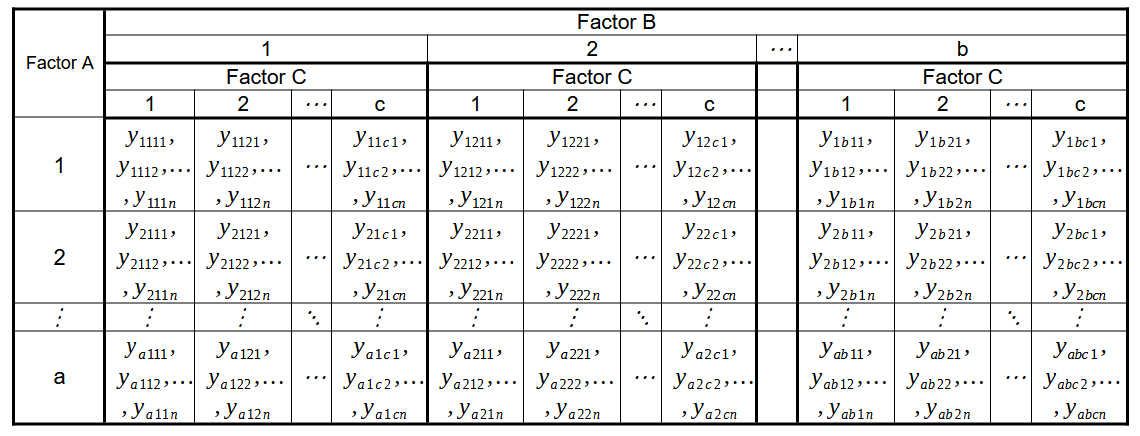
\includegraphics[width=0.90\linewidth]{img/factorial.png} 
	\caption{Disposición general para un diseño factorial con tres factores de efectos fijos.} 
	\label{fig:FactorialTres}
\end{figure}
\FloatBarrier

\textbf{El modelo para un diseño de tres factores es:}\\
	\begin{center}
	$y_{ijkl}=\mu + \tau_{i} + \beta_{j} + \gamma_{k} + (\tau \beta)_{ij} +(\tau \gamma)_{ik} + (\beta \gamma)_{jk} + (\tau \beta \gamma)_{ijk} + \epsilon_{ijkl} $

	$i = 1,2, \dots, a$, $j = 1,2, \dots, b$, $k = 1,2, \dots, c$  y $l = 1,2, \dots, n$
 \end{center}
 
Donde:
\begin{itemize}
	\item $\mu$ es la media general
	\item $\tau_{i}$ efecto del $i$-ésimo nivel del factor renglón $A$.
	\item $\beta_{j}$ efecto del $j$-ésimo nivel del factor columna $B$.
	\item $\gamma_{k} $ efecto del $k$-ésimo nivel del factor columna $C$.
	\item $(\tau \beta)_{ij} $ efecto de la interacción entre $\tau_{i}$  y  $\beta_{j}$ .
	\item $(\tau \gamma)_{ik}$ efecto de la interacción entre  $\tau_{i}$  y  $\gamma_{k}$ .
	\item $(\beta \gamma)_{jk}$ efecto de la interacción entre $\beta_{j}$ y  $\gamma_{k}$ .
	\item $(\tau \beta \gamma)_{ijk}$ efecto de la interacción entre $\tau_{i}$  , $\beta_{j}$ y $\gamma_{k}$ .
	\item $\epsilon_{ijkl}$ es el error aleatorio.
\end{itemize}


\textbf{Supuestos del modelo}\\
 $\epsilon_{ijkl} NI (0, \sigma^{2})$

\textbf{Hipótesis}\\
Para los factores
\begin{center}
	$H^{1}_{0} =\tau_{1} = \tau_{2} = \dots = \tau_{a} = 0$ vs $H^{1}_{1}$ : al menos una $\tau_{i} \neq 0$ , $i = 1,2, \dots, a$ \\
	$H^{2}_{0} =\beta_{1} = \beta_{2} = \dots = \beta_{b} = 0 $ vs $H^{2}_{1}$ : al menos una $\beta_{j} \neq 0$ , $j = 1,2, \dots,b$ \\
	$H^{3}_{0} =\gamma_{1} = \gamma_{2} = \dots = \gamma_{c} = 0 $ vs $H^{3}_{1}$ : al menos una $\gamma_{k} \neq 0$ , $k = 1,2, \dots,c$ \\
\end{center}

Para las interacciones 
\begin{center}
	$H^{4}_{0} : (\tau \beta)_{ij} = 0$ $ \forall i,j$ vs $H^{4}_{1}$ : al menos una $(\tau \beta)_{ij} \neq 0$ , $i = 1,2, \dots, a; j = 1,2, \dots,b$ \\
	$H^{5}_{0} : (\tau \gamma)_{ik} = 0$ $ \forall i,k$ vs $H^{5}_{1}$ : al menos una $(\tau \gamma)_{ik} \neq 0$ , $i = 1,2, \dots, a; k = 1,2, \dots,c$ \\
	$H^{6}_{0} : (\beta \gamma)_{jk} = 0$ $ \forall j,k$ vs $H^{6}_{1}$ : al menos una $(\beta \gamma)_{jk} \neq 0$ , $j = 1,2, \dots, b; k = 1,2, \dots, c$ \\
	$H^{7}_{0} : (\tau \beta \gamma)_{ijk} = 0$ $ \forall i,j,k$ vs $H^{7}_{1}$ : al menos una $(\tau \beta \gamma)_{ijk} \neq 0$ , $i = 1,2, \dots, a; j = 1,2, \dots, b; k = 1,2, \dots, c$ \\
\end{center}

\textbf{Suma de cuadrados}\\
Las fórmulas de cálculo para las sumas de cuadrados son:\\
$ SC_{total} = \sum_{i=1}^{a}  \sum_{j=1}^{b}  \sum_{k=1}^{c}  \sum_{l=1}^{n} y_{ijkl}^{2} - \frac{y_{....}^{2}}{abcn} $\\

$ SC_{A} = \sum_{i=1}^{a} \frac{y_{i...}^{2}}{bcn}  - \frac{y_{....}^{2}}{abcn} $\\

$ SC_{B} = \sum_{j=1}^{b} \frac{y_{.j..}^{2}}{acn}  - \frac{y_{....}^{2}}{abcn} $\\

$ SC_{C} = \sum_{k=1}^{c} \frac{y_{..k.}^{2}}{abn} - \frac{y_{....}^{2}}{abcn} $\\


\textbf{Las sumas de cuadrados para las interacciones son:}\\

$ SC_{AB} = \sum_{i=1}^{a} \sum_{j=1}^{b}  \frac{y_{ij..}^{2}}{cn}  - \frac{y_{....}^{2}}{abcn} - SC_{A} -SC_{B}  $\\

$ SC_{AC} = \sum_{i=1}^{a} \sum_{k=1}^{c}  \frac{y_{i.k.}^{2}}{bn}  - \frac{y_{....}^{2}}{abcn} - SC_{A} -SC_{C}  $\\

$ SC_{BC} = \sum_{j=1}^{b} \sum_{k=1}^{c}  \frac{y_{.jk.}^{2}}{an}  - \frac{y_{....}^{2}}{abcn} - SC_{C} -SC_{B}  $\\


$ SC_{ABC} =  \sum_{i=1}^{a}  \sum_{j=1}^{b}  \sum_{k=1}^{c}  \frac{y_{ijk.}^{2}}{n}  - \frac{y_{....}^{2}}{abcn} - SC_{A} -SC_{B} - SC_{C} -SC_{AB} -SC_{AC} -SC_{BC}  $\\


La suma de cuadrados del error puede encontrarse restando la suma de cuadrados de cada efecto principal e interacción de la suma de cuadrados total:\\

\begin{center}
	$ SC_{E} = SC_{T} -SC_{A} - SC_{B}-SC_{C} -SC_{AB} -SC_{AC} -SC_{BC} -SC_{ABC} $\\
\end{center}

O bien,
\begin{center}
	$ SC_{E} = SC_{T} - SC_{Sub(ABC)} $\\
\end{center}

Donde
\begin{center}
	$ SC_{Sub(ABC)} = \sum_{i=1}^{a}  \sum_{j=1}^{b}  \sum_{k=1}^{c} \frac{y_{ijk.}^{2}}{n} - \frac{y_{....}^{2}}{abcn}  $\\
\end{center}


\textbf{Estadísticos de prueba}\\
Para probar la significación la fuente de variabilidad $X$, se divide $CM_{X}$ por el  $CM_{E}$; de modo que los valores grandes de este cociente implican que los datos no apoyan la hipótesis nula correspondiente:
\begin{center}
	$ F^{X} = \frac{CM_{X}}{CM_{E}} \sim F_{x,abc(n-1)}  $\\
\end{center}


Donde $x$ representa los grados de libertad asociados a la fuente de variabilidad $X$.\\

\textbf{Región de rechazo}\\

Con un nivel de significación dado $\alpha$, la región de rechazo se encuentra en la cola superior de la distribución F correspondiente:

\begin{center}
	$ RR : F_{0}^{X} > F_{a;x,abc(n-1)} $\\
\end{center}

$ F_{0}^{X} $ es el valor de la estadística de prueba correspondiente.

\textbf{Valor p}\\

Se considera la fuente de variación $(X)$ con su correspondiente estadístico de prueba.

\begin{center}
	$ P_{X} =  P( F_{a;x,abc(n-1)} \geq F_{0}^{X} ) $\\
\end{center}


\begin{table}
	\centering
	\begin{tabular}{|c|c|c|c|c|c|}
		\hline
		\makecell{Fuente de \\ variación} & SC & g.l & CM & $F_{0}$ & Valor - p \\ % Encabezados de columna
		\hline
		A & $SC_{A}$ & $a-1$ & $\frac{SC_{A}}{a-1}$ &  $\frac{CM_{A}}{CM_{E}}$ & $P(F \geq F_{0}^{A} )$ \\
		\hline
		B & $SC_{B}$ & $b-1$ & $\frac{SC_{B}}{b-1}$ &  $\frac{CM_{B}}{CM_{E}}$ & $P(F \geq F_{0}^{B} )$ \\
		\hline
		C & $SC_{C}$ & $c-1$ & $\frac{SC_{C}}{c-1}$ &  $\frac{CM_{C}}{CM_{E}}$ & $P(F \geq F_{0}^{C} )$ \\
		\hline
		AB & $SC_{AB}$ & $(a-1)(b-1)$ & $\frac{SC_{AB}}{(a-1)(b-1)}$ &  $\frac{CM_{AB}}{CM_{E}}$ & $P(F \geq F_{0}^{AB} )$ \\
		\hline
		AC & $SC_{AC}$ & $(a-1)(c-1)$ & $\frac{SC_{AC}}{(a-1)(c-1)}$ &  $\frac{CM_{AC}}{CM_{E}}$ & $P(F \geq F_{0}^{AC} )$ \\
		\hline
		BC & $SC_{BC}$ & $(b-1)(c-1) $ & $\frac{SC_{BC}}{(b-1)(c-1)}$ &  $\frac{CM_{BC}}{CM_{E}}$ & $P(F \geq F_{0}^{BC} )$ \\
		\hline
		ABC & $SC_{ABC}$ & $(a-1)(b-1)(c-1)$ & $\frac{SC_{ABC}}{(a-1)(b-1)(c-1)}$ &  $\frac{CM_{ABC}}{CM_{E}}$ & $P(F \geq F_{0}^{ABC} )$ \\
		\hline
		Error & $SC_{E} $ & $abc(n-1)$ & $\frac{SC_{E}}{abc(n-1)}$ & & \\
		\hline
		Total & $SC_{T}$ & $abcn-1$ & & &  \\
		\hline
	\end{tabular}
	\caption{Tabla del ANOVA para el diseño factorial de tres factores con efectos fijos.}
\end{table}
\FloatBarrier

\subsubsection{Comparación múltiple de Tukey}

Si el ANOVA indica que hay diferencia en el nivel medio de los factores resulta de interés llevar a cabo comparaciones entre las medias individuales para determinar diferencias específicas. Existiendo interacción significativa, los efectos de los factores no son independientes.\\


Con la prueba de Tukey el nivel de significación global es exactamente  cuando los tamaños de las muestras son iguales y como máximo $\alpha$ cuando los tamaños de las muestras son desiguales. Este método también puede utilizarse para construir intervalos de confianza sobre las diferencias en todos los pares de medias. Para estos intervalos, el nivel de confianza simultáneo es del $(1-\alpha)100\%$ cuando los tamaños de las muestras son iguales y de al menos $(1-\alpha)100\%$  cuando los tamaños de las muestras son desiguales.\\
%%%Revisar acentos

$H_{0}:\mu_{i} = \mu_{j}$ vs $H_{1}:\mu_{i} \neq \mu_{j}$ para toda $i \neq j$\\

 $\mu_{i} \neq \mu_{j}$ si $| \bar{Y}_{i} -\bar{Y}_{j} | > q_{\alpha} (p,f) \: \sqrt{\frac{CM_{E}}{n}} = T_{\alpha}$ (tamaños de las muestras iguales).\\
 

La tabla V del apéndice en Montgomery (2017) contiene $q_{\alpha} (p,f)$, valor del punto porcentual $\alpha$ superior del estadístico del rango estudentizado $q=\frac{ \bar{Y}_{max} -\bar{Y}_{min}}{ \sqrt{\frac{CM_{E}}{n}}}$, donde $\bar{Y}_{max}$ y $\bar{Y}_{min}$ son las medias muestrales mayor y menor respectivamente de un grupo de $p$ medias muestrales, $f$ son los gl asociados con $CM_{E}$.\\
 
Intervalo de confianza del  $(1-\alpha)100\%$ para $\mu_{i} - \mu_{j}$:\\
 
\begin{center}
	$ \bar{Y}_{max} -\bar{Y}_{min} -  q_{\alpha} (p,f) \: \sqrt{\frac{CM_{E}}{n}} \leq \mu_{i} - \mu_{j} \leq \bar{Y}_{max} -\bar{Y}_{min} + q_{\alpha} (p,f) \: \sqrt{\frac{CM_{E}}{n}} $ \\
\end{center}

Para tamaños de muestras desiguales, en la prueba de hipótesis se utiliza:\\

\begin{center}
	$ T_{\alpha} = \frac{q_{\alpha} (p,f)}{\sqrt{2}} \sqrt{CM_{E} (\frac{1}{n_{i}} + \frac{1}{n_{j}})}  $ \\
\end{center}


Los intervalos de confianza para la diferencia de los pares de medias se determinan con:\\


\begin{center}
	$ \bar{Y}_{max} -\bar{Y}_{min} -  \frac{q_{\alpha} (p,f)}{\sqrt{2}} \sqrt{CM_{E} (\frac{1}{n_{i}} + \frac{1}{n_{j}})}  \leq \mu_{i} - \mu_{j} \leq \bar{Y}_{max} -\bar{Y}_{min} + \frac{q_{\alpha} (p,f)}{\sqrt{2}} \sqrt{CM_{E} (\frac{1}{n_{i}} + \frac{1}{n_{j}})}  $ \\
\end{center}

A la versión para tamaños de las muestras diferentes se llama el procedimiento de Tukey-Kramer.
